\chapter{BIODATA PENULIS}

\begin{wrapfigure}{l}{0.3\textwidth}
	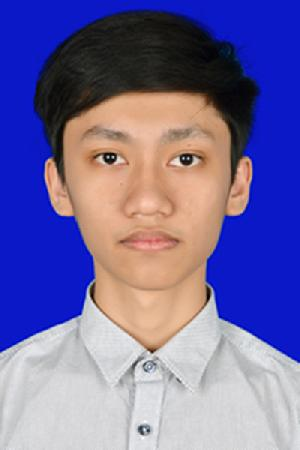
\includegraphics[height=0.3\textheight]{penutup/img/foto.jpeg}
\end{wrapfigure}

Penulis bernama Michael Julian Albertus, putra kedua dari tiga bersaudara yang lahir pada tanggal 2 Juli 1998 di Pekanbaru. Penulis telah mengenyam pendidikan di Sekolah Dasar Mardi Yuana Serang pada tahun 2004 hingga 2006, Sekolah Dasar Palm Kids pada tahun 2006 hingga 2009, Sekolah Dasar Negeri 005 Sukajadi Pekanbaru pada tahun 2009 hingga 2010, Sekolah Menengah Pertama Negeri 5 Pekanbaru pada tahun 2010 hingga 2013, dan Sekolah Menengah Atas Negeri 8 Pekanbaru pada tahun 2013 hingga 2015. Pada masa penulisan, penulis sedang menempuh masa studi S1 di Institut Teknologi Sepuluh Nopember, Surabaya di \jurusan.

Selama masa studi, penulis memiliki ketertarikan yang dalam mengenai \textit{artificial intelligence}, \textit{competitive programming}, dan rancang bangun aplikasi sistem informasi. Keinginan penulis dalam mengajar juga mendorong penulis menjadi asisten dosen pada mata kuliah Dasar Pemrograman, Struktur Data, dan Sistem Operasi. Karya penulis semasa perkuliahan diantaranya adalah pembangunan SheNeedsLab dan LPencerdas untuk acara Hackathon. Selama menempuh perkuliahan penulis juga aktif mengikuti kompetisi pemrograman tingkat nasional dan menjadi finalis pada lomba pemrograman COMPFEST (2017, 2018, dan 2019), INC Bina Nusantara (2017, 2018, dan 2019), FINDIT 2019, Arkavidia (2017,2018, dan 2019) dan menjadi Juara 3 HOLOGY 2018.

Di luar kesibukan akademik, penulis juga berkontribusi dalam berbagai kepanitiaan, baik dalam skala kecil (yaitu dalam kampus) maupun skala nasional. Kepanitian yang penulis ikuti adalah Schematics (2017 dan 2018). Kegiatan terakhir penulis adalah membantu kegiatan pelatihan nasional bagi peserta Olimpiade Komputer Indonesia pada Februari dan Maret 2019 lalu. Penulis dapat dihubungi melalui surel di michaeljulian98@gmail.com.

